% Section content template for individual Educative lessons
% This file contains the actual content for a specific section
% Generated from Educative API section content

% Section: System Design: The Distributed Search
% Section ID: 5400897294696448
% Section Slug: system-design-the-distributed-search
% Generated: 2025-12-07T21:51:02.838828

\subsection{Why do we need a search system?}\label{hLzhBIlNUr162qT-lhS6i}
\\
Nowadays, we see a search bar on almost every website. We use that search bar to pick out relevant content from the enormous amount of content available on that website. A search bar enables us to quickly find what we're looking for. For example, there are plenty of courses present on the Educative website. If we didn't have a search feature, users would have to scroll through many pages and read the name of each course to find the one they're looking for.

\begin{figure}[htbp]
 \centering
 
\includegraphics[width=0.15\textwidth]{Images/chapter_21/section_5400897294696448/4637132253954048.png}
 
\end{figure}

Let's take another example. There are billions of videos uploaded and stored on YouTube. Imagine if YouTube didn\textquotesingle t provide us with a search bar. How would we find a specific video among the millions of videos that have been posted on YouTube over the years? It would take months to navigate through all of those videos and find the one we need. Users find it challenging to find what they're looking for simply by scrolling around.
\\
Search engines are an even bigger example. We have billions of websites on the Internet. Each website has many web pages and there is plenty of content on each of these web pages. With so much content, the Internet would practically be useless without search engines, and users would end up lost in a sea of irrelevant data. Search engines are, essentially, filters for the massive amount of data available. They let users quickly obtain information that is of true interest without having to sift through too many unnecessary web pages.\\
\strut \\
Behind every search bar, there is a search system.

\subsection{What is a search system?}\label{lLqtTCM6w8XqDGUBJvR_l}
\\
A \textbf{search system} is a system that takes some text input, a search query, from the user and returns the relevant content in a few seconds or less. There are three main components of a search system, namely:

\begin{itemize}
\item
\protect\phantomsection\label{QesQB958uge9o0TPeInHV}
A \textbf{crawler}, which fetches content and creates documents(For a search engine, a document consists of the text extracted from a web page. In a movie store's web page, a document could be a JSON object containing titles, descriptions, and other metadata of the videos upon which we want to perform search queries. The documents could be JSON or any other suitable format. Documents are stored on a distributed storage like S3 or HDFS.).
\item
\protect\phantomsection\label{nC9saaN5CTFj3BzvldFGc}
An \textbf{indexer}, which builds a searchable index.
\item
\protect\phantomsection\label{_nq13Iz3KRgYzgHcsrSP8}
A \textbf{searcher}, which responds to search queries by running the search query on the \emph{index} created by the \emph{indexer}.
\end{itemize}

\begin{figure}[htbp]
 \centering
 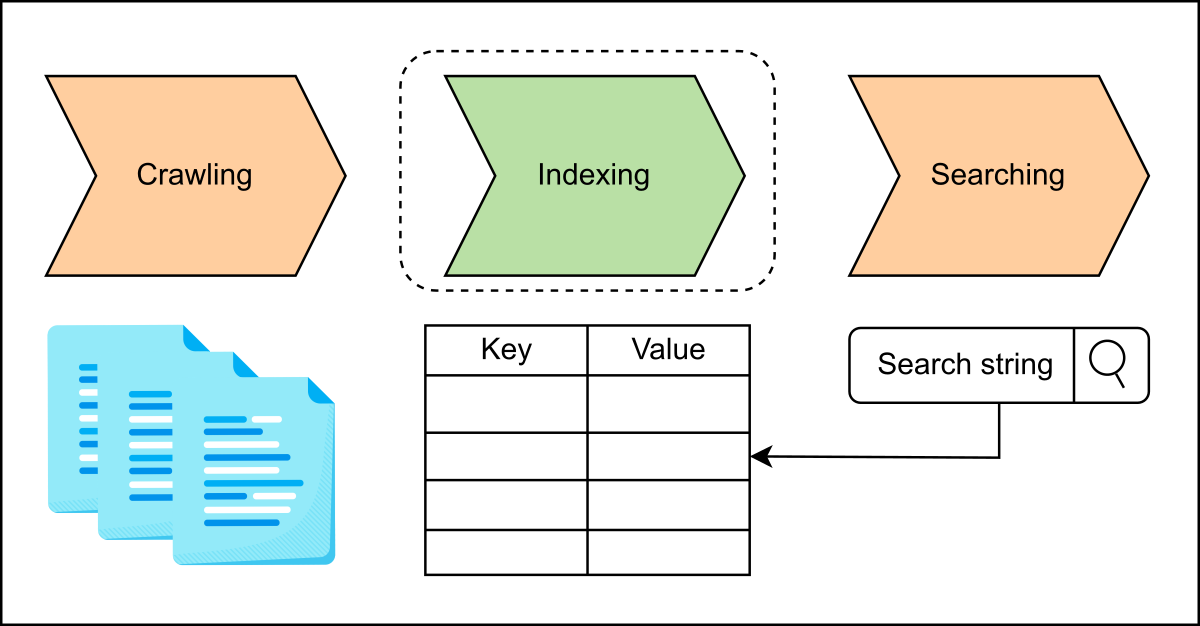
\includegraphics[width=0.5\textwidth]{Images/chapter_21/section_5400897294696448/5366455063674880.png}
 \caption{The three phases of a search system}
\end{figure}

\textbf{Note:} We have a separate chapter dedicated to the explanation of the \href{https://www.educative.io/courses/grokking-the-system-design-interview/system-design-web-crawler}{crawler} component. In this chapter, we'll focus on indexing.

\subsection{How will we design a distributed search system?}\label{Hl5nYuNAP2Na4cIDQs8Ds}
\\
We divided the design of a distributed search system into five lessons:

\begin{enumerate}
\item
\protect\phantomsection\label{PescbaozFXHv9bdbGk3iv}
\href{https://www.educative.io/courses/grokking-the-system-design-interview/requirements-of-a-distributed-search-systems-design}{\textbf{Requirements:}} In this lesson, we list the functional and non-functional requirements of a distributed search system. We also estimate our system's resources, such as servers, storage, and the bandwidth needed to serve a number of queries.
\item
\protect\phantomsection\label{y-NhRRh39Re8_Uy6PMH1T}
\href{https://www.educative.io/courses/grokking-the-system-design-interview/indexing-in-a-distributed-search}{\textbf{Indexing:}} This lesson provides us with background knowledge on the process of indexing with the help of an example. After discussing indexing, we also look into a centralized architecture of distributed search systems.
\item
\protect\phantomsection\label{I_SQQ8a2cppduvKuFNPKc}
\href{https://www.educative.io/courses/grokking-the-system-design-interview/design-of-a-distributed-search}{\textbf{Initial design:}} This lesson consists of the high-level design of our system, its API, and the details of the indexing and searching process.
\item
\protect\phantomsection\label{S9zclZXmGsl3jH8348v2S}
\href{https://www.educative.io/courses/grokking-the-system-design-interview/scaling-search-and-indexing}{\textbf{Final design:}} In this lesson, we evaluate our previous design and revamp it to make it more scalable.
\item
\protect\phantomsection\label{HsdcZBXfhl4GQ_FeKviWV}
\href{https://www.educative.io/courses/grokking-the-system-design-interview/evaluation-of-a-distributed-searchs-design}{\textbf{Evaluation:}} This lesson explains how our designed distributed search system fulfills its requirements.
\end{enumerate}
\\
Let's start by understanding the requirements of designing a distributed search system.

% End of section content